\documentclass{beamer}
\usepackage{tikz}
\usepackage{filecontents}
\usetikzlibrary{calc}

\begin{filecontents*}{table_data.tex}
  \begin{tabular}{l*{3}{c}}
    & A & B & C \\
    \hline
    \textbf<2>{1} & blah & blah & blah \\
    2 & blah & blah & blah \\
    3 & blah & blah & blah \\
    \hline
  \end{tabular}
\end{filecontents*}

\begin{document}
\begin{frame}
  \begin{center}
    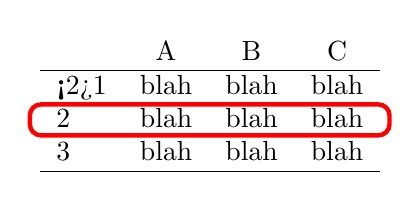
\begin{tikzpicture}
      \node (table) {  \begin{tabular}{l*{3}{c}}
    & A & B & C \\
    \hline
    \textbf<2>{1} & blah & blah & blah \\
    2 & blah & blah & blah \\
    3 & blah & blah & blah \\
    \hline
  \end{tabular}
};
      \draw [red,ultra thick,rounded corners]
      ($(table.south west) !.3! (table.north west)$) rectangle ($(table.south east) !.5! (table.north east)$);
    \end{tikzpicture}
  \end{center}
\end{frame}
\end{document}
